\chapter{Tests}

\section{Schematics}

float barrier command to ensure that text stays close to the picture but no text from after the picture.

\subsection{part 1}

\begin{figure}[ht]
    \centering
    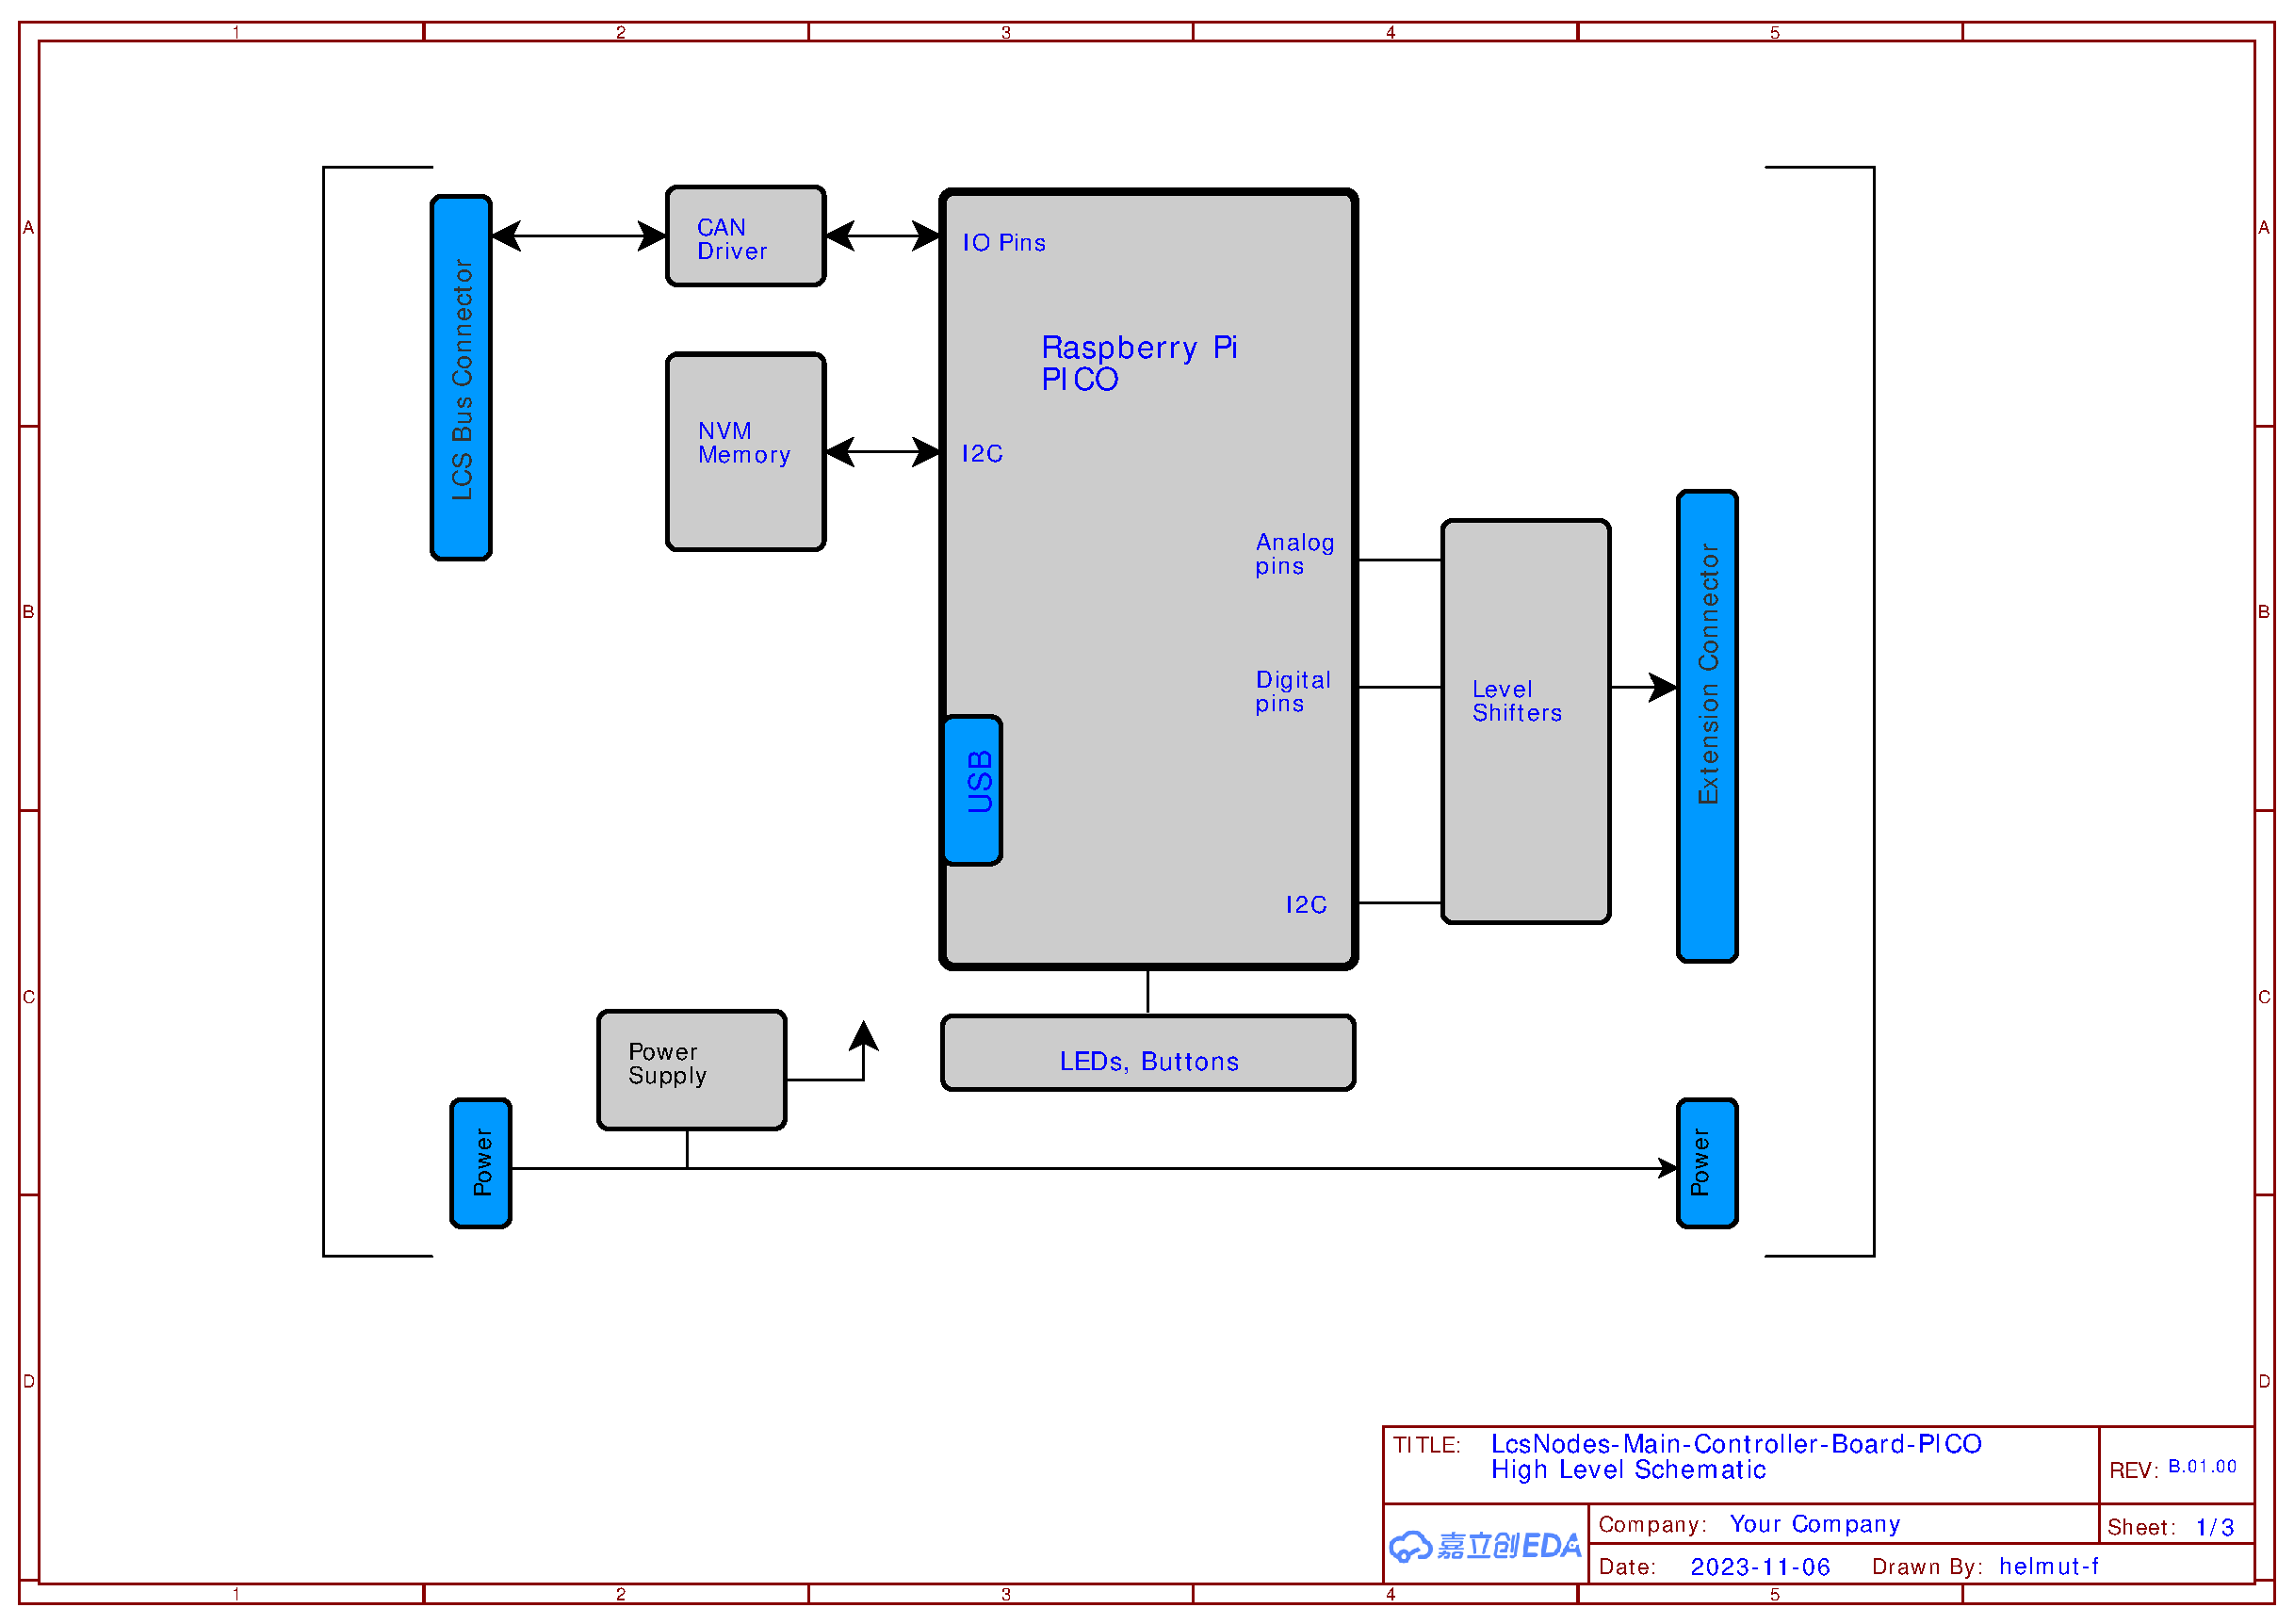
\includegraphics[page=1, width=\textwidth]{./schematics/Schematic_LcsNodes-Main-Controller-Board.pdf}
\end{figure}

\FloatBarrier

\subsection{part 2}
\begin{figure}[ht]
    \centering
    \includegraphics[page=2, width=\textwidth]{./schematics/Schematic_LcsNodes-Main-Controller-Board.pdf}
\end{figure}

\FloatBarrier

\subsection{part 3}
\begin{figure}[ht]
    \centering
    \includegraphics[page=3, width=\textwidth]{./schematics/Schematic_LcsNodes-Main-Controller-Board.pdf}
\end{figure}

\FloatBarrier


\section{Pictures}

\subsection{An instruction word layout}

A little test for an instruction word layout ... will be a bit fiddling work ... 

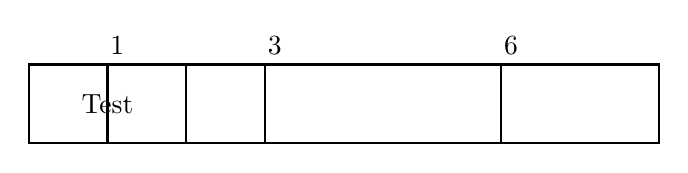
\begin{tikzpicture}
    \draw[thick] (0, 0) rectangle (8, 1); % Simple rectangle
    \node at (1, 0.5) {Test};   % Centered text
    \draw[thick] (2, 0) -- (2, 1);

    \foreach \x in {1, 3, 6} {
        \draw[thick] (\x, 0) -- (\x, 1); % Vertical line
        \node[above] at (\x + 0.125, 1) {\x}; % a number above the field
    }

\end{tikzpicture}


% example for the protocol chapter... instead of the tables....

\section{Protocol boxes}

A bit cumbersome and we would need to have text at defined locations. Perhaps keep the simple table in the protocol chapter.

\begin{center}
\begin{tikzpicture}

    \draw[help lines, gray!50, dashed] (0,0) grid( 16,8);

    \node[  draw, 
            rectangle, 
            minimum width=6cm, 
            minimum height=4cm, 
            text height=1cm, 
            align=left] (A) at (4, 4) 
            { };

    \node[  draw, 
            rectangle, 
            minimum width=6cm, 
            minimum height=4cm, 
            text height=1cm, 
            align=left] (B) at (12, 4) 
            { };

    \draw[->] (A.north east) ++(0, -1) -- ($(B.west) + (0, 1 )$);
    \draw[->] (B.south west) ++(0,  1) -- ($(A.east) + (0, -1)$);

    \node at ( 4,  6.25 ) {\textbf{Node A}};
    \node at ( 12, 6.25 ) {\textbf{Node B}};

    \node at ( 2.25,  5 ) {\textbf{LCS\_TOF}};
    \node at ( 10.25, 3 ) {\textbf{LCS\_TOF}};

\end{tikzpicture}
\end{center}



\section{Split rectangle}

We would need the split rectangle for the runtime area maps....

\begin{tikzpicture}

    \draw[help lines, gray!50, dashed] (0,0) grid(16,12);

    \node at (3, 3.0) {Hugo};
    \node at (3, 1.5) {Berta};
    \node at (3, 0.5) {Carla};

    \node[  tsRectangle, 
            minimum width=6cm,
            minimum height=10cm,
            fill=yellow!50] (nvm) at (4,5) {};

    \draw[draw](1,2) -- (7,2);
    \draw[draw](1,2) -- (7,2);
    \draw[draw](1,2) -- (7,2);
    \draw[draw](1,2) -- (7,2);
   
    \node[  tsRectangle, 
            minimum width=6cm,
            minimum height=10cm,
            fill=yellow!50] (mem) at (13,5) {};


\end{tikzpicture}

